\documentclass[12pt]{article}

\usepackage{../preamble}

\title{topology}
\author{Runi Malladi}

\begin{document}
\maketitle

\section{metric spaces} % {{{1 

\begin{definition}
	Let $(X,d)$ be a metric space. A \emph{curve} in $X$ is a continuous mapping $\gamma: [0,1] \to X$. 
\end{definition}

\begin{definition}
	Let $\gamma$ be a curve in $(X,d)$. Let $P[0,1]$ denote the set of partitions of $[0,1]$. For each $\mathcal{P}\in P[0,1]$, with components $p_0 < \cdots < p_n$, define 
	\begin{equation*}
		\ell_\mathcal{P}(\gamma) = \sum_{i=1}^n d(\gamma(p_{i-1}), \gamma(p_i)).
	\end{equation*}
	The \emph{length} of $\gamma$ is 
	\begin{equation*}
		\ell(\gamma) = \sup_\mathcal{P} \ell_\mathcal{P}(\gamma).
	\end{equation*}
\end{definition}

\begin{proposition}
	\begin{equation*}
		\lim_{|\mathcal{P}|\to 0} \ell_\mathcal{P}(\gamma) = \ell(\gamma).
	\end{equation*}
\end{proposition}
\begin{proof}
	Fix $\epsilon>0$. We need to find $\delta>0$ such that $\ell(\gamma) - \epsilon < \ell_{\mathcal{Q}}(\gamma) \leq \ell(\gamma)$. By the definition of the supremum, there exists $\mathcal{P}\in P[0,1]$ such that 
	\begin{equation*}
		\ell(\gamma)-\epsilon < \ell_\mathcal{P}(\gamma) \leq \ell(\sigma).
	\end{equation*}
	Let $\epsilon'>0$ be arbitrary. Since $\sigma$ is continuous on a compact space, it is uniformly continuous (REF), hence there exists $\eta>0$ such that $|t-t'|<\eta$ implies $d(\gamma(t),\gamma(t'))<\epsilon'$ for all $t,t'\in [0,1]$. Let $\delta=\min(\eta, |\mathcal{P}|)$.

	Suppose $\mathcal{Q}\in P[0,1]$ is such that $|\mathcal{Q}|<\delta$. Say it is given by $q_0<\cdots <q_m$. Let $\mathcal{R}=\mathcal{P}\cup\mathcal{Q}$. For each $i=1,\dots, n$, there exists a finite set $\{r_{i,k}\}_{k=0}^{K_i}\subset\mathcal{R}$ partitioning $[p_{i-1}, p_i]$. Then 
	\begin{align*}
		\ell_\mathcal{R}(\gamma)) 
		=& \sum_{i=1}^n \sum_{k=1}^{K_i} d(\gamma(r_{i, k-1}, \gamma(i, r_k))) \\
		\leq& \sum_{i=1}^n d(\gamma(\max_{q_j\leq r_{i,0}}q_j), \gamma(r_{i,0})) + \sum_{k=1}^{K_i}d(\gamma(r_{i,k-1}),\gamma(r_{i,k})) + d(\gamma(r_{i,K_i}), \gamma(\min_{q_j\geq r_{i,K_i}}q_j)) \\
		\leq& \sum_{i=1}^n d(\gamma(\max_{q_j\leq r_{i,0}}q_j), \gamma(\min_{q_j\geq r_{i,K_i}}q_j)) \\
		\leq& \ell_\mathcal{Q}(\gamma) + 2n\epsilon'.
	\end{align*}
	Figure \ref{fig_arclength_overlap_strat} demonstrates our strategy here.
	
	\begin{figure}
		\label{fig_arclength_overlap_strat}
		\centering
		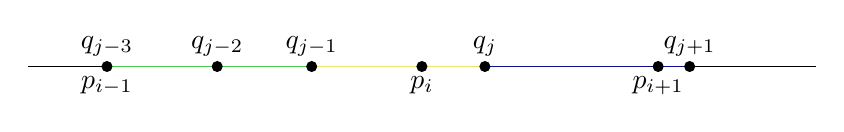
\begin{tikzpicture}
			\coordinate (A) at (-5,0);
			\coordinate (pim1) at (-4,0);
			\coordinate (qjm2) at (-2.6,0);
			\coordinate (qjm1) at (-1.4,0);
			\coordinate (pi) at (0,0);
			\coordinate (qj) at (0.8,0);
			\coordinate (pip1) at (3,0);
			\coordinate (qjp1) at (3.4,0);
			\coordinate (B) at (5,0);

			% Draw the line
			\draw (A) -- (B);

			% Draw the colored segments
			\draw[green] (pim1) -- (qjm1);
			\draw[blue] (qj) -- (qjp1);
			\draw[yellow] (qjm1) -- (qj);

			% Label the points
			\fill (pim1) circle (2pt) node[below] {$p_{i-1}$} node[above] {$q_{j-3}$};
			\fill (qjm2) circle (2pt) node[above] {$q_{j-2}$};
			\fill (qjm1) circle (2pt) node[above] {$q_{j-1}$};
			\fill (pi) circle (2pt) node[below] {$p_{i}$};
			\fill (qj) circle (2pt) node[above] {$q_{j}$};
			\fill (pip1) circle (2pt) node[below] {$p_{i+1}$};
			\fill (qjp1) circle (2pt) node[above] {$q_{j+1}$};

		\end{tikzpicture}
		\caption{This is an example of what $\mathcal{P}\cup\mathcal{Q}$ could look like. The green line extends from $q_{j-3}$ to $q_j$ and represents the domain of one summand, and the blue line extends from $q_{j-1}$ to $q_{j+1}$ and represents the next summand. The yellow line from $q_{j-1}$ to $q_j$ represents the overlap; this region is ``double counted''.}
	\end{figure}

	Now 
	\begin{gather*}
		\ell(\gamma)-\epsilon < \ell_\mathcal{P}(\gamma) \leq \ell_\mathcal{R}(\gamma) \leq \ell_\mathcal{Q}(\gamma) + 2n\epsilon', \\
		\ell_\mathcal{R}(\gamma) - 2n\epsilon' \leq \ell_\mathcal{Q}(\gamma).
	\end{gather*}
	But our choice of $\epsilon'$ was arbitrary; if we pick, say,
	\begin{equation*}
		\epsilon' = \frac{1}{2n} \cdot \frac{\ell_\mathcal{P}(\gamma)-(\ell(\gamma)-\epsilon)}{4}
	\end{equation*}
	then we can choose $\delta$ in such a way that that, whenever $|\mathcal{Q}|<\delta$, we have 
	\begin{equation*}
		\ell(\gamma)-\epsilon < \ell_\mathcal{P}(\gamma)-2n\epsilon' \leq \ell_\mathcal{Q}(\gamma) < \ell(\gamma)
	\end{equation*}
	as desired.
\end{proof}

\begin{proposition}
	Let $s(t) = \ell(\gamma|_{[0,t]})$ for $0\leq t\leq 1$. Then $s$ is continuous.
\end{proposition}
\begin{proof}
	Let $\{t_n\}_1^\infty$ be a convergent sequence in $[0,1]$ with limit $t$. Then 
	\begin{align*}
		\lim_{n\to \infty} s(t_n) 
		=& \lim_{n\to\infty} \ell(\gamma|_{[0,t]}) \\
		=& \lim_{n\to\infty} \lim_{|\mathcal{P}_n|\to 0, \mathcal{P}_n\in P[0,t_n]} \ell_{\mathcal{P}_n}(\gamma) \\
		=& \lim_{|\mathcal{P}|\to 0, \mathcal{P}\in P[0,t]} \ell_\mathcal{P}(t) = \ell(\sigma|_{[0,t]}) \\\
		=& s(t).
	\end{align*}
\end{proof}


% metric spaces }}}1

\end{document}
